% ***************************************************************************************************
%
%	Szablon pracy magisterskiej dla Politechniki Wrocławskiej w wersji dwustronnej.
%	Autor:	Tomasz Strzałka
%
% ***************************************************************************************************

% Styl dwustronny z domyślną wielkością czcionki 10pt oraz oddzieloną stroną tytułową (titlepage).
% Domyślnie rodziały rozpoczynają się na stronie prawej (openright).
\documentclass{book}

% ***************************************************************************************************
% Ustawienia języka
% ***************************************************************************************************

% Podstawowe ustawienia języka, według którego formatowany będzie dokument
\usepackage[polish]{babel}

% Pakiet babel dla polskiego języka powoduje konflikt z pakietem amssymb.
% Polecenie '\lll' definiują oba pakiety - porządana jest druga definicja.
\let\lll\undefined

% W przypadku wielojęzykowości ustawia główny język dokumentu
\selectlanguage{polish}

% Kodowanie dokumentu
\usepackage[utf8]{inputenc}

% Dowolny rozmiar czcionek, kodowanie znaków
\usepackage{lmodern}

% Polskie wcięcia akapitów
\usepackage{indentfirst}

% Polskie łamanie wyrazów
\usepackage[plmath]{polski}

% Przecinek w wyrażeniach matematycznych zamiast kropki
\usepackage{icomma}

% Polskie formatowanie typograficzne
\frenchspacing

% Zapewnia liczne usprawnienia wyświetlania i organizacji matematycznych formuł. 
\usepackage{amsmath}

% Wprowadza rozszerzony zestaw symboli m.in. \leadsto
\usepackage{amssymb}

% Dodatkowa, ,,kręcona'' czcionka matematyczna
\usepackage{mathrsfs}

% Dodatkowe wsparcie dla środowiska mathbb, które nie wspiera domyślnie cyfr (\mathbb{})
\usepackage{bbold}

% Fixes/improves amsmath
\usepackage{mathtools}


% ***************************************************************************************************
% Kolory  
% ***************************************************************************************************

% Umożliwia kolorowanie poszczególnych komórek tabeli
\usepackage[table]{xcolor}% http://ctan.org/pkg/

% Umożliwia łatwą zmianę koloru linii w tabeli
\usepackage{tabu}

% Umożliwia rozszerzoną kontrolę nad kolorami.
\usepackage{xcolor}

% Definicje kolorów
\definecolor{lgray}{HTML}{9F9F9F}
\definecolor{dgray}{HTML}{5F5F5F}
% lgray				-	nazwa nowo zdefiniowanego koloru
% HTML				-	model kolorów
% CCCCCC			-	wartość koloru zgodna z modelem

% ***************************************************************************************************
% Algorytmy 
% ***************************************************************************************************

% Udostępnia środowisko do konstruowania pseudokodów
\usepackage[ruled,vlined,linesnumbered,longend,algochapter]{algorithm2e}
% ruled	- poziome kreski na początku i końcu algorytmu, podpis na górze oddzielony również kreską poziomą
% vlined - pionowe kreski łączące początek polecenia z jego końcem
% linesnumbered	- numerowanie kolejnych wierszy algorytmu
% longend - długie końcówki np. ifend, forend itd.
% algochapter - numeracja z rozdziałami

% Zamiana nazwy środowiska z domyślnej "Algorithm X" na "Pseudokod X"
\newenvironment{pseudokod}[1][htb]{
	\renewcommand{\algorithmcfname}{Pseudokod}
	\begin{algorithm}[#1]%
	}{
\end{algorithm}
}

% Zmiana rozmiaru komentarzy
\newcommand\algcomment[1]{
	\footnotesize{#1}
}

% Ustawienie zadanego stylu dla komentarzy
\SetCommentSty{algcomment}

% Wyśrodkowana tylda
\usepackage{textcomp}%
\newcommand{\textapprox}{\raisebox{0.5ex}{\texttildelow}}

% Listowanie kodów źródłowych
\usepackage{listings} 
\renewcommand{\lstlistingname}{Kod źródłowy} % Polska nazwa listingu

% Definicje pecjalnych znaków, które nie są obsługiwane w środowisku listing
\lstset{literate=
	{ż}{{\.{z}}}1	{ź}{{\'{z}}}1
	{ć}{{\'{c}}}1	{ń}{{\'{n}}}1
	{ą}{{\c a}}1	{ś}{{\'{s}}}1
	{ł}{{\l}}1		{ę}{{\c{e}}}1
	{ó}{{\'{o}}}1	{á}{{\'a}}1
	{é}{{\'e}}1		{í}{{\'i}}1
	{ó}{{\'o}}1		{ú}{{\'u}}1
	{ù}{{\`u}}1		{Á}{{\'A}}1
	{É}{{\'E}}1		{Í}{{\'I}}1
	{Ó}{{\'O}}1		{Ú}{{\'U}}1
	{à}{{\`a}}1		{è}{{\'e}}1
	{ì}{{\`i}}1		{ò}{{\`o}}1
	{ò}{{\`o}}1		{À}{{\`A}}1
	{È}{{\'E}}1		{Ì}{{\`I}}1
	{Ò}{{\`O}}1		{Ò}{{\`O}}1
	{ä}{{\"a}}1		{ë}{{\"e}}1
	{ï}{{\"i}}1		{ö}{{\"o}}1
	{ü}{{\"u}}1		{Ä}{{\"A}}1
	{Ë}{{\"E}}1		{Ï}{{\"I}}1
	{Ö}{{\"O}}1		{Ü}{{\"U}}1
	{â}{{\^a}}1		{ê}{{\^e}}1
	{î}{{\^i}}1		{ô}{{\^o}}1
	{û}{{\^u}}1		{Â}{{\^A}}1
	{Ê}{{\^E}}1		{Î}{{\^I}}1
	{Ô}{{\^O}}1		{Û}{{\^U}}1
	{œ}{{\oe}}1		{Œ}{{\OE}}1
	{æ}{{\ae}}1		{Æ}{{\AE}}1
	{ß}{{\ss}}1		{ç}{{\c c}}1
	{Ç}{{\c C}}1	{ø}{{\o}}1
	{å}{{\r a}}1	{Å}{{\r A}}1
	{€}{{\EUR}}1	{£}{{\pounds}}1
}

% ***************************************************************************************************
% Marginesy 
% ***************************************************************************************************

% Ustawienia rozmiarów stron i ich marginesów
\usepackage[headheight=18pt, top=25mm, bottom=25mm, left=25mm, right=25mm]{geometry}
% headheight		-	wysokość tytułów
% top				-	margines górny
% bottom			-	margines dolny
% left				-	margines lewy
% right				-	margines prawy

% Usunięcie górnego marginesu dla środowisk
\makeatletter
\setlength\@fptop{0\p@}	
\makeatother

% ***************************************************************************************************
% Styl 
% ***************************************************************************************************

% Definiuje środowisko 'titlingpage', które zapewnia pełną kontrolę nad układem strony tytułowej.
\usepackage{titling}


% Umożliwia modyfikowanie stylu spisu treści
\usepackage{tocloft}	

\tocloftpagestyle{tableOfContentStyle}

% Definiowanie własnych stylów nagłówków i/lub stopek
\usepackage{fancyhdr}

% Domyślny styl dla pracy 
\fancypagestyle{custom}{
	\fancyhf{}									% wyczyść stopki i nagłówki
	\fancyhead[RO]{								% Prawy, nieparzysty nagłówek
		\hrulefill \hspace{16pt} \large Rozdział \thechapter
		\put(-472.1, 12.1){%
			\makebox(0,0)[l]{%
				
\includegraphics[width=0.05\textwidth]{pwr-logo}
			}
		}
		\put(-443,5.5){%
			\makebox(0,0)[l]{%
				\small Politechnika Wrocławska
			}
		}
	}
	\fancyhead[LE]{								% Lewy, parzysty nagłówek
		\large Rozdział \thechapter \hspace{16pt} \hrulefill 
		\put(-22, 12.1){%
			\makebox(0,0)[l]{%
				
\includegraphics[width=0.05\textwidth]{wppt-logo}
			}
		}
		\put(-210,5.5){%
			\makebox(0,0)[l]{%
				\small Wydział Podstawowych Problemów Techniki
			}
		}
	}
	\fancyfoot[LE,RO]{							% Stopki
		\thepage
	}
	\renewcommand{\headrulewidth}{0pt}			% Grubość linii w nagłówku
	\renewcommand{\footrulewidth}{0.2pt}		% Grubość linii w stopce
}


% Domyślny styl dla bibliografii
\fancypagestyle{bibliographyStyle}{
	\fancyhf{}									% wyczyść stopki i nagłówki
	\fancyhead[RO]{								% Prawy, nieparzysty nagłówek
		\hrulefill \hspace{16pt} \large Dodatek \thechapter
		\put(-472.1, 12.1){%
			\makebox(0,0)[l]{%
				
\includegraphics[width=0.05\textwidth]{pwr-logo}
			}
		}
		\put(-443,5.5){%
			\makebox(0,0)[l]{%
				\small Politechnika Wrocławska
			}
		}
	}
	\fancyhead[LE]{								% Lewy, parzysty nagłówek
		\large Bibliografia \hspace{16pt} \hrulefill 
		\put(-22, 12.1){%
			\makebox(0,0)[l]{%
				
\includegraphics[width=0.05\textwidth]{wppt-logo}
			}
		}
		\put(-210,5.5){%
			\makebox(0,0)[l]{%
				\small Wydział Podstawowych Problemów Techniki
			}
		}
	}
	\fancyfoot[LE,RO]{							% Stopki
		\thepage
	}
	\renewcommand{\headrulewidth}{0pt}			% Grubość linii w nagłówku
	\renewcommand{\footrulewidth}{0.2pt}		% Grubość linii w stopce
}

% Domyślny styl dla dodatków
\fancypagestyle{appendixStyle}{
	\fancyhf{}									% wyczyść stopki i nagłówki
	\fancyhead[RO]{								% Prawy, nieparzysty nagłówek
		\hrulefill \hspace{16pt} \large Dodatek \thechapter
		\put(-472.1, 12.1){%
			\makebox(0,0)[l]{%
				
\includegraphics[width=0.05\textwidth]{pwr-logo}
			}
		}
		\put(-443,5.5){%
			\makebox(0,0)[l]{%
				\small Politechnika Wrocławska
			}
		}
	}
	\fancyhead[LE]{								% Lewy, parzysty nagłówek
		\large Dodatek \thechapter \hspace{16pt} \hrulefill 
		\put(-22, 12.1){%
			\makebox(0,0)[l]{%
				
\includegraphics[width=0.05\textwidth]{wppt-logo}
			}
		}
		\put(-210,5.5){%
			\makebox(0,0)[l]{%
				\small Wydział Podstawowych Problemów Techniki
			}
		}
	}
	\fancyfoot[LE,RO]{							% Stopki
		\thepage
	}
	\renewcommand{\headrulewidth}{0pt}			% Grubość linii w nagłówku
	\renewcommand{\footrulewidth}{0.2pt}		% Grubość linii w stopce
}

% Osobny styl dla stron zaczynających rozdział/spis treści itd. (domyślnie formatowane jako "plain")
\fancypagestyle{chapterBeginStyle}{
	\fancyhf{}%
	\fancyfoot[LE,RO]{
		\thepage
	}
	\renewcommand{\headrulewidth}{0pt}
	\renewcommand{\footrulewidth}{0.2pt}
}

% Styl dla pozostałych stron spisu treści
\fancypagestyle{tableOfContentStyle}{
	\fancyhf{}%
	\fancyfoot[LE,RO]{
		\thepage
	}
	\renewcommand{\headrulewidth}{0pt}
	\renewcommand{\footrulewidth}{0.2pt}
}

% Formatowanie tytułów rozdziałów i/lub sekcji
\usepackage{titlesec}

% Formatowanie tytułów rozdziałów
\titleformat{\chapter}[hang]					% kształt
{
	\vspace{-10ex}
	\Huge
	\bfseries
}												% formatowanie tekstu modyfikowanego elementu
{}												% etykieta występująca przed tekstem modyfikowanego elementu, niewidoczna w spisie treści
{
	10pt
}												% odstęp formatowanego tytułu od lewego marginesu/etykiety
{
	\Huge
	\bfseries
}												% formatowanie elementów przed modyfikowanym tytułem
[
\vspace{2ex}
%\rule{\textwidth}{0.4pt}
%\vspace{-4ex}
]												% dodatkowe formatowanie stosowane poniżej modyfikowanego tytułu


% Formatowanie tytułów sekcji
\titleformat{\section}[hang]					% kształt
{
	\vspace{2ex}
%	\titlerule\vspace{1ex}
	\Large\bfseries
}												% formatowanie tekstu modyfikowanego elementu
{
	\thesection									% etykieta występująca przed tekstem modyfikowanego elementu, niewidoczna w spisie treści
}
{
	0pt
}												% odstęp formatowanego tytułu od lewego marginesu/etykiety
{
	\Large
	\bfseries
}												% formatowanie elementów przed modyfikowanym tytułem

% ***************************************************************************************************
% Linki
% ***************************************************************************************************

% Umożliwia wstawianie hiperłączy do dokumentu
\usepackage{hyperref}							% Aktywuje linki

\hypersetup{
	colorlinks	=	true,					% Koloruje tekst zamiast tworzyć ramki.
	linkcolor		=	blue,					% Kolory: referencji,
        citecolor		=	blue,					% cytowań,
	urlcolor		=	blue					% hiperlinków.
}

% Do stworzenia hiperłączy zostanie użyta ta sama (same) czcionka co dla reszty dokumentu
\urlstyle{same}




% ***************************************************************************************************
% Linki
% ***************************************************************************************************

% Umożliwia zdefiniowanie własnego stylu wyliczeniowego
\usepackage{enumitem}

% Nowa lista numerowana z trzema poziomami
\newlist{myitemize}{itemize}{3}

% Definicja wyglądu znacznika pierwszego poziomu
\setlist[myitemize,1]{
	label		=	\textbullet,
	leftmargin	=	4mm}

% Definicja wyglądu znacznika drugiego poziomu
\setlist[myitemize,2]{
	label		=	$\diamond$,
	leftmargin	=	8mm}

% Definicja wyglądu znacznika trzeciego poziomu
\setlist[myitemize,3]{
	label		=	$\diamond$,
	leftmargin	=	12mm
}

% ***************************************************************************************************
% Inne pakiety
% ***************************************************************************************************

% Dołączanie rysunków
\usepackage{graphicx}

% Figury i przypisy
\usepackage{caption}
\usepackage{subcaption}

% Umożliwia tworzenie przypisów wewnątrz środowisk
\usepackage{footnote}

% Umożliwia tworzenie struktur katalogów
\usepackage{dirtree}

% Rozciąganie komórek tabeli na wiele wierszy
\usepackage{multirow}

% Precyzyjne obliczenia szerokości/wysokości dowolnego fragmentu wygenerowanego przez LaTeX
\usepackage{calc}

% ***************************************************************************************************
% Matematyczne skróty
% ***************************************************************************************************

% Skrócony symbol liczb rzeczywistych
\newcommand{\RR}{\mathbb{R}}

% Skrócony symbol liczb naturalnych
\newcommand{\NN}{\mathbb{N}}

% Skrócony symbol liczb wymiernych
\newcommand{\QQ}{\mathbb{Q}}

% Skrócony symbol liczb całkowitych
\newcommand{\ZZ}{\mathbb{Z}}

% Skrócony symbol logicznej implikacji
\newcommand{\IMP}{\rightarrow}

% Skrócony symbol  logicznej równoważności
\newcommand{\IFF}{\leftrightarrow}

% ***************************************************************************************************
% Środowiska
% ***************************************************************************************************

% Środowisko do twierdzeń
\newtheorem{theorem}{Twierdzenie}[chapter]

% Środowisko do lematów
\newtheorem{lemma}{Lemat}[chapter]

% Środowisko do przykładów
\newtheorem{example}{Przykład}[chapter]

% Środowisko do wniosków
\newtheorem{corollary}{Wniosek}[chapter]

% Środowisko do definicji
\newtheorem{definition}{Definicja}[chapter]

% Środowisko do dowodów
\newenvironment{proof}{
	\par\noindent \textbf{Dowód.}
}{
\begin{flushright}
	\vspace*{-6mm}\mbox{$\blacklozenge$}
\end{flushright}
}

% Środowisko do uwag
\newenvironment{remark}{
	\bigskip \par\noindent \small \textbf{Uwaga.}
}{
\begin{small}
	\vspace*{4mm}
\end{small}
}

% ***************************************************************************************************
% Słownik
% ***************************************************************************************************

% Prawidłowe dzielenie wyrazów
\hyphenation{wszy-stkich ko-lu-mnę każ-da od-leg-łość
	dzie-dzi-ny dzie-dzi-na rów-nych rów-ny
	pole-ga zmie-nna pa-ra-met-rów wzo-rem po-cho-dzi
	o-trzy-ma wte-dy wa-run-ko-wych lo-gicz-nie
	skreś-la-na skreś-la-ną cał-ko-wi-tych wzo-rów po-rzą-dek po-rząd-kiem
	przy-kład pod-zbio-rów po-mię-dzy re-pre-zen-to-wa-ne
	rów-no-waż-ne bi-blio-te-kach wy-pro-wa-dza ma-te-ria-łów
	prze-ka-za-nym skoń-czo-nym moż-esz na-tu-ral-na cią-gu tab-li-cy
	prze-ka-za-nej od-po-wied-nio}

% ***************************************************************************************************
% Dokument
% ***************************************************************************************************

\frontmatter

\begin{document}

	\begin{titlingpage}
		\vspace*{\fill}
		\begin{center}
			\begin{picture}(300,510)
				\put(11,520){\makebox(0,0)[l]{\large \textsc{Wydział Podstawowych Problemów Techniki}}}
				\put(11,500){\makebox(0,0)[l]{\large \textsc{Politechnika Wrocławska}}}
% Tytuł pracy
                \put(80,280){\Huge \textsc{Redundantny}}
                        \put(80,240){\Huge \textsc{system plików}}
% Autor pracy
				\put(90,200){\makebox(0,0)[l]{\large \textsc{Kacper Pieniążek}}}
				\put(90,180){\makebox(0,0)[l]{\large \textsc{Nr indeksu: 236606}}}

				\put(200,100){\makebox(0,0)[l]{\large Praca inżynierska napisana}}
				\put(200,80){\makebox(0,0)[l]{\large pod kierunkiem}}
% dane promotora
				\put(200,60){\makebox(0,0)[l]{\large dra Macieja Gębali}}
				
				\put(115,-70){
\includegraphics[width=0.15\textwidth]{pwr}}
				\put(106,-80){\makebox(0,0)[bl]{\large \textsc{Wrocław 2019}}}
			\end{picture}
		\end{center}	
		\vspace*{\fill}
	\end{titlingpage}
	
        \cleardoublepage
		
	\pagenumbering{Roman}
	\pagestyle{tableOfContentStyle}
	\tableofcontents
	\cleardoublepage
		
	% ***************************************************************************************************
	% Wstęp
	% ***************************************************************************************************
	
	\pagestyle{custom}
	\mainmatter
	
	% ***************************************************************************************************
	% Rodziały
	% ***************************************************************************************************

	\chapter{Wstęp}
\thispagestyle{chapterBeginStyle}

Praca dyplomowa swoim zakresem obejmuje detekcję i korekcję błędów, niezawodność danych oraz wybrane metody redundancji. Celem pracy jest zaprojektowanie i implementacja systemu plików o następujących założeniach:
\begin{itemize}
    \item Detekcja błędów w plikach
    \item Korekcja znalezionych błędów
    \item Zapisywanie wielu kopii danych
    \item Odzyskiwanie utraconych danych 
\end{itemize}

Chociaż istnieją systemy plików umożliwiające zarówno odzyskiwanie, jak i zabezpieczanie danych przed uszkodzeniami\cite{Java}, omawiany projekt w założeniu działa inaczej niż znalezione systemy. Przeważnie redundantne systemy plików są tworzone z myślą o grupach dysków, łącząc je we wspólną jednostkę logiczną. Zastosowane rozwiązania do odzyskiwania danych są często zakorzenione głęboko w logice takie systemu, znacząco utrudniając wprowadzanie nowych rozwiązań.

Praca składa się z czterech rozdziałów. W rozdziale pierwszym poddano szczegółowej analizie metody detekcji oraz korekcji błędów, rozważono istniejące modele podziału oraz kopiowania danych i przedstawiono rozwiązania wykorzystane w implementowanym systemie.

W rozdziale drugim wykorzystano scenariusze do opisania działania systemu oraz zabrazowano wybrane zagadnienia przy pomocy diagramów. Algorytmy wykorzystane w projekcie zostały przedstawione w pseudokodzie wraz z opisem rozwiązania.

W rozdziale trzecim opisano technologie implementacji projektu. Przedstawiono strukturę kodu źródłowego oraz omówiono wybrane szczegóły implementacji.

W rozdziale czwartym przedstawiono sposób instalacji i zamontowania systemu w środowisku docelowym. Opisano przykładowe metody użycia oraz załączone testy systemu.


	\cleardoublepage

	\chapter{Analiza problemu}
\thispagestyle{chapterBeginStyle}
\label{rozdzial1}

Analiza problemu
---------------------------------
W tym rozdziale należy przedstawić analizę zagadnienia, które podlega informatyzacji. Należy zidenty-
fikować i opisać obiekty składowe rozważanego wycinka rzeczywistości i ich wzajemne relacje (np. użytkown-
ików systemu i ich role). Należy szczegółowo omówić procesy jakie zachodzą w systemie i które będą infor-
matyzowane, takie jak np. przepływ dokumentów. Należy sprecyzować i wypunktować założenia funkcjon-
alne i poza funkcjonalne dla projektowanego systemu. Jeśli istnieją aplikacje realizujące dowolny podzbiór
zadanych funkcjonalności realizowanego systemu należy przeprowadzić ich analizę porównawczą, wskazując na
różnice bądź innowacyjne elementy, które projektowany w pracy system informatyczny będzie zawierał. Należy
odnieść się do uwarunkowań prawnych związanych z procesami przetwarzania danych w projektowanym sys-
temie. Jeśli zachodzi konieczność, należy wprowadzić i omówić model matematyczny elementów systemu na
odpowiednim poziomie abstrakcji.
{\color{dgray}
W niniejszym rozdziale omówiono koncepcję architektury programowej systemu \ldots. W
szczególny sposób \ldots. Omówiono założenia funkcjonalne i niefunkcjonalne podsystemów \ldots. Przedstawiono
mechanizmy \ldots. Sklasyfikowano systemy ze względu na \ldots. Omówiono istniejące rozwiązania informatyczne o podobnej funkcjonalności \ldots (zobacz \cite{JCINodesChord}).

-Omowienie sposobow redundancji danych -RAID -Istniejace rozwiazania -Wybrane rozwiazania
-Problem rozbijania danych -Problem wielu replik -Problem synchronizacji -Problem obsługi pełnej funkcjon-
alności, np. softlinks
Założenia: -Rodzaj wykorzystywanego sposobu redundacji niewidoczny dla uzytkownika -Uzytkownik nie
martwi sie replikami poza wyjatkowymi sytuacjami: synchronizacja replik przy zamontowaniu, zatwierdzenie
korekty
}

\begin{itemize}
    \item Obsługa kilku różnych rozwiązań redundancji
    \item Obsługa wielu replik dla większego bezpieczeństwa danych 
    \item Wybór najodpowiedniejszej repliki do odczytu danych
    \item Synchronizacja istniejących danych pomiędzy replikami przy zamontowaniu systemu plików
	\item Obsługa przynajmniej podstawowych zachowań systemu plików:
		\begin{itemize}
			\item Czytanie oraz pisanie do plików
			\item Tworzenie oraz usuwanie plików
		\end{itemize}
	\item Detekcja błędów:
		\begin{itemize}
			\item Sprawdzanie, czy pliki, na których dokonywane są operacje, nie są uszkodzone
			\item Sprawdzanie synchronizacji danych między replikami
		\end{itemize}
	\item Korekcja błędów:
		\begin{itemize}
			\item Zastosowanie kodów korekcyjnych
			\item Całkowite zastępowanie uszkodzonych danych replikami
		\end{itemize}
    \item Wygoda uzytkowania
\end{itemize}

\section {Redundancja danych}
Redundancja danych stanowi najwazniejsze zagadnienie rozwazanej pracy. Zaproponowano kilka roznych rozwiazan, aby przedstawic pozadany zakres mozliwosci systemu. Rozwiazania oparte sa na macierzy RAID ze wzgledu na ich skutecznosc oraz mozliwosc tworzenia kombinacji standardowych poziomow.

wspomniec o tym ze pomimo nazwy replika mozna miec np jedna i to ma zerowa redundancje ew korekte
\subsection {RAID}
Redundant Array of Independent Disks to metoda wirtualizacji przechowywania danych. Wykorzystuje wiele dyskow i laczy je w logiczne jednostki pamieci. RAID jest stosowane do redundancji danych oraz lepszej wydajnosci, jednak w niniejszej pracy wydajnosc systemu nie bedzie rozwazana.  
RAID jest zbiorem schematow rozwiazan, ktore nazywane sa poziomami. Na potrzeby pracy przedstawione zostana wybrane poziomy, ktore wprowadzaja rozne metody redundancji.
\subsubsection{Poziom 0}
\begin{figure}[h!]
        \centering
        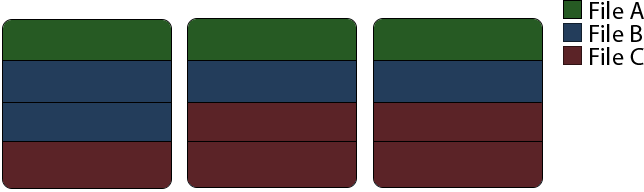
\includegraphics{raid-0.png}
        \caption{RAID-0 z trzema dyskami}
        \label{fig:raid0}
\end{figure}
\subsubsection{Poziom 1}
\begin{figure}[h!]
        \centering
        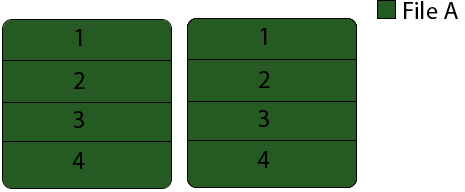
\includegraphics{raid-1.png}
        \caption{RAID-1 z dwoma dyskami}
        \label{fig:raid1}
\end{figure}
\subsubsection{Poziom 2}
dupa
\begin{figure}[h!]
        \centering
        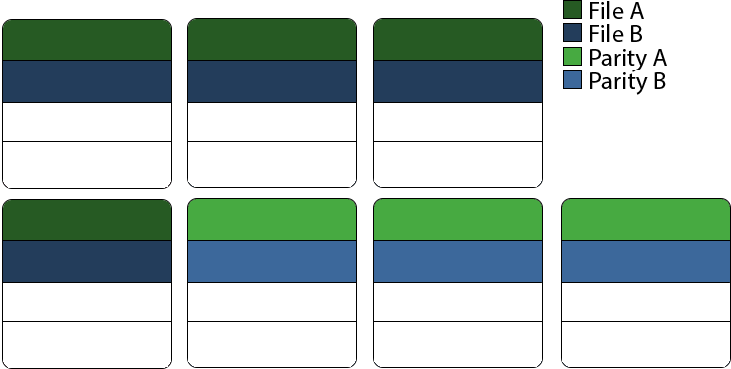
\includegraphics{raid-2.png}
        \caption{RAID-2 na siedmiu dyskach}
        \label{fig:raid2}
\end{figure}
\subsubsection{Poziom 4}
dupa
\begin{figure}[h!]
        \centering
        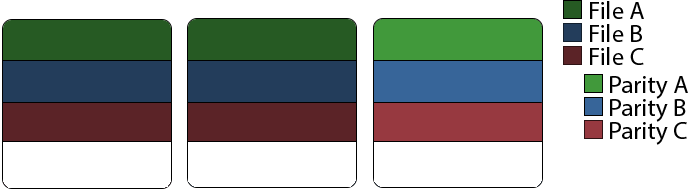
\includegraphics{raid-4.png}
        \caption{RAID-4 na trzech dyskach}
        \label{fig:raid4}
\end{figure}
\subsubsection{Poziom 5}
dupa
\begin{figure}[h!]
        \centering
        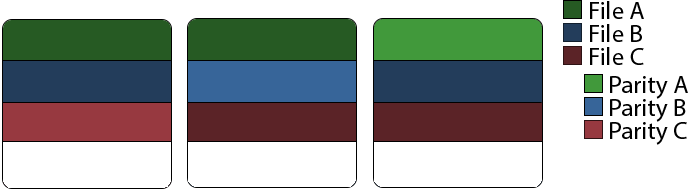
\includegraphics{raid-5.png}
        \caption{RAID-5 na trzech dyskach}
        \label{fig:raid5}
\end{figure}
\subsubsection{Poziom 6}
dupa

\newpage
\subsection{Standardowe repliki systemu}
Repliki zostaly zaprojektowane na podstawie poziomow RAID. Roznia sie miedzy soba sposobem wprowadzenia redundancji danych oraz mozliwym zastosowaniem. Ponizej opisano proponowane rodzaje replik oraz rozwazono ich mocne i slabe strony. Wszystkie rodzaje mozna podzielic na dwie kategorie:
\begin{itemize}
    \item Replika standardowa - Dokonuje detekcji bledow w plikach, jednak w przypadku wykrycia takiego bledu lub desynchronizacji z innymi replikami, nie jest w stanie dokonac korekty bledow bez dodatkowych replik
    \item Replika korekcyjna - Dokonuje zarowno detekcji, jak i korekcji znalezionych bledow. Jesli korekta znalezionych bledow jest niemozliwa, zachowuje sie podobnie do repliki bez korekty - desynchronizacja moze zostac naprawiona wylacznia z dodatkowymi replikami
\end{itemize}
Repliki korekcyjne dodają funkcjonalność do standardowej, dlatego zostały omówione w późniejszej sekcji pracy. 

\subsubsection{Repliki Lustrzane (MR)}
Oparte na schemacie RAID-1 repliki tego typu stanowią lustrzane odbicie danych. Funkcjonalność takie systemu jest równa systemowi nadrzędnemu. 
\begin{itemize}
        \item Naprawia błędy innych replik kopiując całe pliki
        \item Wszystkie dane zamontowane w jednym miejscu. W przypadku, kiedy jeden dysk zostanie uszkodzony, dane zostają utracone.
\end{itemize}

\begin{figure}[h!]
        \centering
        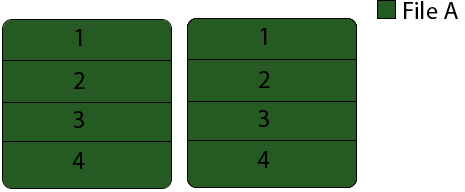
\includegraphics{raid-1.png}
        \caption{Dwie repliki blokowe}
        \label{fig:raid1}
\end{figure}

Standardowe MR nie są w stanie naprawić uszkodzonych plików. Jedynym rozwiązaniem jest zastąpić uszkodzone pliki w całości danymi z innej repliki. Niestandardowymi MR nazywa się repliki lustrzane z korektą błędów.
\subsubsection{Repliki Blokowe (BR)}
W replikach tego typu pliki są rozkładane na części i zapisywane w kolejnych katalogach będących odpowiednikiem dysków poziomu RAID-0. Tak samo katalogi mogą być rozmieszczone na różnych urządzeniach przechowujących. Każdy z katalogów może również być repliką. Jedna część pliku nazywana jest dalej blokiem.
Rozkład danych jest możliwy na dwa sposoby:
\begin{itemize}
    \item Pliki podzielone na stałą ilość bloków o zmiennych wielkościach. 

            Zmiana wielkości pliku może powodować zmianę rozmiaru wszystkich bloków danego pliku dla wyrównania wielkości, lub jedynie tego bloku, do którego dane zostają dopisane. W takim wypadku bloki nie są jednakowych rozmiarów.
            \begin{figure}[h!]
                    \centering
                    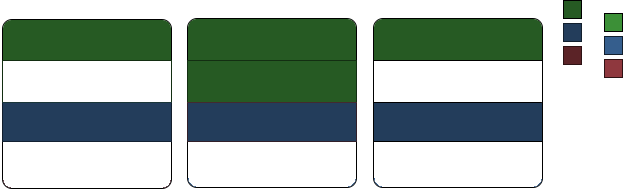
\includegraphics{BR-1.png}
                    \caption{Podział pliku na trzy nierówne bloki }
                    \label{fig:br1}
            \end{figure}
    \item Pliki podzielone na zmienną ilość części o ograniczonych wielkościach

            Określony jest maksymalny dozwolony rozmiar dla pojedynczego bloku. Przy przekroczeniu rozmiaru bloku, system tworzy kolejny w następnym katalogu dopóki jest miejsce. 
            \begin{figure}[h!]
                    \centering
                    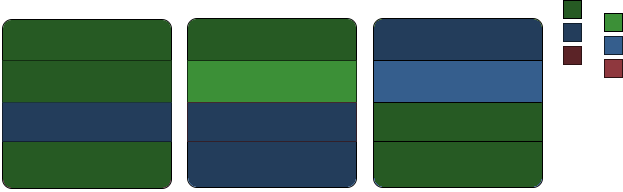
\includegraphics{BR-2.png}
                    \caption{Podzial pliku na wiele bloków ograniczonego rozmiaru}
                    \label{fig:br1}
            \end{figure}
 
\end{itemize}
Standardowe BR nie są w stanie naprawić uszkodzonych plików, jednak taki podział danych wpłynie korzystnie na repliki korekcyjne i jest szczególnie przydatny dla wielu dysków.
\begin{itemize}
    \item Naprawia błędy innych replik kopiując jedynie częściowe pliki, jeśli to możliwe.
    \item Dane mogą zostać zamontowane w wielu miejscach. W przypadku uszkodzenia jednego dysku, reszta danych jest nadal dostępna.
\end{itemize}

\subsection{Podzial replik na warstwy}

\section {Korekcja błędów}
\subsection{Kod Hamminga}
\subsection{Parzystość bloku}
\subsection{Repliki korekcyjne}

Dodanie metod korekcji błędów w replikach BR umożliwi odzyskiwanie całych bloków. W przypadku uszkodzonego dysku, repliki BR mogą być w stanie zmienić lokalizację odzyskanego bloku lub zmienić sposób, w jaki dzielą dane. To znaczy, że jeśli replika blokowa działa na n dyskach, działa również po awarii na n-1 dyskach dla n < 1.

\section {Detekcja błędów}

\section {Synchronizacja replik}

\section {Dzialanie systemu plikow}

\section {Wygoda uzytkowania}

	\cleardoublepage

	\chapter{Projekt systemu}
\thispagestyle{chapterBeginStyle}
W tym rozdziale przedstawiono scenariusze oraz przypadki uzycia systemu, na koncu znajduje sie diagram przedstawiajacy zachowanie systemu w okreslonych sytuacjach. Omowiono i przedstawiono w postaci pseudokodu algorytmy zastosowane w systemie. 

\section{Grupy użytkowników i założenia}

{\color{dgray}
Architektura systemu \ldots jest wielowarstwowa i rozproszona, przy czym \ldots. Podsystem  \ldots jest systemem zbiorczym dla danych \ldots wysyłanych do serwera \ldots. 

Taka architektura jest zgodna z wzorcem projektowym MVC\footnote{Należy odnieść się do wykorzystywanych wzorców projektowych} (ang.  Model-View-Controller). Przetwarzanie danych odbywa się \ldots.
} 

\section{Przypadki użycia i scenariusze}
\subsection{Montowanie systemu plików}
\begin{table}[h!]
        \centering
        \begin{tabular}{ |l|p{10cm}| }
                \hline
            S01 & Montowanie systemu plików \\ \hline
            Aktor & Użytkownik \\ \hline
            Warunki wsępne & Aktor przygotował konfigurację systemu \\ \hline
            & \\ Przebieg wydarzeń & \textbullet Aktor montuje system, podając plik konfiguracyjny \newline \newline 
            \textbullet System odczytuje konfigurację \newline \newline 
            \textbullet System dostosowuje parametry i montuje system plików \\
            & \\ \hline
            Alternatywny przebieg wydarzeń & \textbullet Aktor konfiguruje system przez argumenty wywołania \\ \hline
            Sytuacje wyjątkowe & \textbullet Aktor podał niepoprawną konfigurację \newline \newline
            \textbullet Katalogi podane przez aktora nie istnieją lub są niepoprawne \\ \hline
            Warunki końcowe & System plików jest poprawnie zamontowany pod podanym katalogiem \\ \hline
        \end{tabular}
        \caption{Montowanie systemu plików}
\end{table}
\newpage

\subsection{Odczyt pliku}
\begin{table}[h!]
        \centering
        \begin{tabular}{ |l|p{10cm}| }
                \hline
            S02.1 & Odczyt pliku przy wykorzystaniu pojedynczej repliki korekcyjnej \\ \hline
            Aktor & Użytkownik \\ \hline
            Warunki wsępne & System plików jest zamontowany, replika wspiera korekcję błędów \\ \hline
            Przebieg wydarzeń & 
            1. Aktor podaje plik do odczytu \newline \newline 
            2. System sprawdza spójność pliku w replice \newline \newline 
            3. System dokonuje korekty istniejących uszkodzeń pliku przed odczytem danych \newline \newline
            4. Aktor dostaje odczytane dane \\ \hline
            Alternatywny przebieg wydarzeń & 
            3. System nie może dokonać korekty błędów  \newline \newline
            4. Aktor zostaje poinformowany o błędzie \newline \newline
            5. Aktor dostaje odczytane dane\\ \hline
            Sytuacje wyjątkowe & \textbullet Dany plik nie istnieje w replice  \newline \newline
            \textbullet Nieudany odczyt pliku \newline \newline
            \textbullet Dysk z repliką został odmontowany lub uszkodzony \\ \hline
            Warunki końcowe & System zwrócił aktorowi odczytane dane \\ \hline
        \end{tabular}
        \caption{Odczyt pliku przy wykorzystaniu pojedynczej repliki korekcyjnej}
\end{table}

\begin{table}[h!]
        \centering
        \begin{tabular}{ |l|p{10cm}| }
                \hline
            S02.2 & Odczyt pliku przy wykorzystaniu pojedynczej repliki standardowej  \\ \hline
            Aktor & Użytkownik \\ \hline
            Warunki wstępne & System plików jest zamontowany, replika nie wspiera korekty błędów \\ \hline
            Przebieg wydarzeń & 
            1. Aktor podaje plik do odczytu \newline \newline 
            2. System sprawdza spójność pliku w replice \newline \newline
            3. System informuje o znalezionych błędach \newline \newline
            4. Aktor dostaje odczytane dane \\ \hline
            Alternatywny przebieg wydarzeń & 
            Brak\\ \hline
            Sytuacje wyjątkowe & \textbullet Dany plik nie istnieje w replice  \newline \newline
            \textbullet Błąd oczytu \newline \newline
            \textbullet Dysk z repliką został odmontowany lub uszkodzony \\ \hline
            Warunki końcowe & System zwrócił aktorowi odczytane dane \\ \hline
        \end{tabular}
        \caption{Odczyt pliku przy wykorzystaniu pojedynczej standardowej repliki}
\end{table}

\newpage
\begin{table}[h!]
        \centering
        \begin{tabular}{ |l|p{10cm}| }
                \hline
            S02.4 & Odczyt pliku przy wykorzystaniu wielu replik\\ \hline
            Aktor & Użytkownik \\ \hline
            Warunki wstępne & System plików jest zamontowany, wiele replik aktywnych \\ \hline
            Przebieg wydarzeń & 
            1. Aktor podaje plik do odczytu \newline \newline 
            2. System odczytuje plik z najlepszej repliki\newline \newline
            3. System naprawia uszkodzenia odczytując dane z innych replik \newline \newline
            4. Aktor dostaje odczytane dane \\ \hline
            Alternatywny przebieg wydarzeń & 
            4. Dane w replice nie zostały naprawione \newline \newline
            5. System wyłącza replikę \\ \hline
            Sytuacje wyjątkowe & \textbullet Dany plik nie istnieje w replice  \newline \newline
            \textbullet Błąd oczytu \newline \newline
            \textbullet Replika jest jedyną działającą \\ \hline
            Warunki końcowe & System zwrócił aktorowi odczytane dane i replika została naprawiona lub wyłączona \\ \hline
        \end{tabular}
        \caption{Odczyt pliku przy wykorzystaniu wielu replik}
\end{table}

\begin{table}[h!]
        \centering
        \begin{tabular}{ |l|p{10cm}| }
                \hline
            S02.5 & Odczyt brakujacego pliku w replice\\ \hline
            Aktor & Użytkownik \\ \hline
            Warunki wstępne & System plików jest zamontowany \\ \hline
            Przebieg wydarzeń & 
            1. Aktor podaje plik do odczytu \newline \newline 
            2. System wykrywa brak pliku \newline \newline
            3. System sprawdza obecnosc pliku w pozostalych replikach \newline \newline
            4. Brakujace dane zostaja zsynchronizowane miedzy replikami\\ \hline
            Alternatywny przebieg wydarzeń & 
            \textbullet Brak innych replik \newline \newline
            \textbullet Brak pliku we wszystkich replikach \\ \hline
            Sytuacje wyjątkowe & 
            \textbullet Błąd oczytu \newline \newline
            \textbullet Jedyna istniejaca kopia pliku jest zbyt uszkodzona\\ \hline
            Warunki końcowe & System zwrócił aktorowi odczytane dane i dane zostaly zsynchronizowane lub aktor zostal poinformowany o braku pliku\\ \hline
        \end{tabular}
        \caption{Odczyt brakujacego pliku w replice}
\end{table}

\newpage


\subsection{Zapis pliku}
\begin{table}[h!]
        \centering
        \begin{tabular}{ |l|p{10cm}| }
                \hline
            S03.1 & Zapis pliku przy wykorzystaniu pojedynczej repliki korekcyjnej \\ \hline
            Aktor & Użytkownik \\ \hline
            Warunki wstępne & System plików jest zamontowany, replika wspiera korekcję błędów \\ \hline
            Przebieg wydarzeń & 
            1. Aktor podaje dane do zapisu \newline \newline 
            2. System dopisuje dodatkowe informacje do korekty \newline \newline 
            3. System zapisuje do repliki \\ \hline
            Alternatywny przebieg wydarzeń &
            4. System nie może dopisać dodatkowych informacji  \newline \newline
            5. System zwraca błąd zapisu \\ \hline
            Sytuacje wyjątkowe & 
            \textbullet Nieudany zapis pliku \newline \newline
            \textbullet Dysk z repliką został odmontowany lub uszkodzony \newline \newline
            \textbullet Brak miejsca na replice \\ \hline
            Warunki końcowe & System zapisał dane podane przez aktora oraz informacje do korekcji \\ \hline
        \end{tabular}
        \caption{Zapis pliku przy wykorzystaniu pojedynczej repliki korekcyjnej} 
\end{table}

\begin{table}[h!]
        \centering
        \begin{tabular}{ |l|p{10cm}| }
                \hline
                S03.2 & Zapis pliku przy wykorzystaniu pojedynczej repliki standardowej\\ \hline
            Aktor & Użytkownik \\ \hline
            Warunki wstępne & System plików jest zamontowany, replika nie wspiera korekcji błędów \\ \hline
            Przebieg wydarzeń & 
            1. Aktor podaje dane do zapisu \newline \newline
            2. System dopisuje dodatkowe informacje do detekcji bledow \newline \newline
            2. System zapisuje do repliki \\ \hline
            Alternatywny przebieg wydarzeń &
            3. System nie może zapisać do repliki  \newline \newline
            4. System zwraca błąd zapisu \\ \hline
            Sytuacje wyjątkowe & 
            \textbullet Nieudany zapis pliku \newline \newline
            \textbullet Dysk z repliką został odmontowany lub uszkodzony \newline \newline
            \textbullet Brak miejsca na replice \\ \hline
            Warunki końcowe & System zapisał dane podane przez aktora \\ \hline
        \end{tabular}
        \caption{Zapis pliku przy wykorzystaniu pojedynczej repliki standardowej}
\end{table}
\newpage

\begin{table}[h!]
        \centering
        \begin{tabular}{ |l|p{10cm}| }
                \hline
            S03.3 & Zapis pliku przy wykorzystaniu wielu replik\\ \hline
            Aktor & Użytkownik \\ \hline
            Warunki wstępne & System plików jest zamontowany, wiele replik \\ \hline
            Przebieg wydarzeń & 
            1. Aktor podaje dane do zapisu \newline \newline 
            2. System zapisuje dane do każdej repliki \newline \newline 
            3. Każdy błąd zapisu wyłącza daną replikę\\ \hline
            Alternatywny przebieg wydarzeń &
            Brak \\ \hline
            Sytuacje wyjątkowe & 
            \textbullet Nieudany zapis pliku do każdej repliki\newline \newline
            \textbullet Wszystkie repliki zostały wyłączone \\ \hline
            Warunki końcowe & System zapisał dane podane przez aktora i są działające repliki\\ \hline
        \end{tabular}
        \caption{Zapis pliku przy wykorzystaniu wielu replik} 
\end{table}

\subsection {Niezorganizowane}
\begin{table}[h!]
        \centering
        \begin{tabular}{ |l|p{10cm}| }
                \hline
            S04.1 & Wybor najlepszej repliki\\ \hline
            Aktor & Użytkownik \\ \hline
            Warunki wstępne & System plików jest zamontowany, przynajmniej jedna replika\\ \hline
            Przebieg wydarzeń & 
            1. System sprawdza czy sa aktywne repliki \newline \newline 
            2. System wybiera najlepsza replike z aktywnych \\ \hline
            Alternatywny przebieg wydarzeń &
            Brak \\ \hline
            Sytuacje wyjątkowe & 
            \textbullet Wszystkie repliki zostały wyłączone \\ \hline
            Warunki końcowe & System wybral replike i wykonuje operacje aktora\\ \hline
        \end{tabular}
        \caption{Wybor najlepszej repliki} 
\end{table}



\newpage





\section{Diagramy}

\section{Opis algorytmów}

W tej sekcji należy wymienić i przedyskutować algorytmy wykorzystywane w systemie. Algorytmy należy przedstawić w pseudokodzie (wykorzystać pakiet \texttt{algorithm2e}). Omówienia poszczególnych kroków algorytmów powinny zawierać odwołania do odpowiednich linii pseudokodu. Dla zaproponowanych autorskich algorytmów należy przeprowadzić analizę ich złożoności czasowej i pamięciowej. 

~\ref{alg:mine}.

{\small
\begin{pseudokod}[H]
%\SetAlTitleFnt{small}
\SetArgSty{normalfont}
\SetKwFunction{Process}{Process}
\SetKwFunction{Calculate}{Calculate}
\KwIn{Zbiór bąbli $B$}
\KwOut{Wyporność $W$}
\ForEach{$b \in B$}{
\Process{$b$}\;
\For{$i \leftarrow 1$ \KwTo $|B|$}{
\If{\Calculate{EW($i$,$b$)} $\le$ 0}{
$b \leftarrow 2*b$\;
}
}
}
\While{$B \neq \emptyset$}{
\For{$j \leftarrow 1$ \KwTo $|B|$}{
\If{\Calculate{FT($j$,$\hat{b}$)} $\le 0$}{
$w \leftarrow 2*\hat{b}$\;
$W \leftarrow W \cup \{w\}$\;
$B \leftarrow B \setminus \{b\}$\;
}
}
}
\caption{Wybor najlepszej repliki}\label{alg:mine}
\end{pseudokod}
}

{\small
\begin{pseudokod}[H]
%\SetAlTitleFnt{small}
\caption{Kodowanie Huffmana}\label{alg:mine}
\end{pseudokod}
}

{\small
\begin{pseudokod}[H]
%\SetAlTitleFnt{small}
\caption{Obliczanie parzystosci dla danych}\label{alg:mine}
\end{pseudokod}
}

{\small
\begin{pseudokod}[H]
%\SetAlTitleFnt{small}
\caption{Odzyskiwanie pliku}\label{alg:mine}
\end{pseudokod}
}

{\small
\begin{pseudokod}[H]
%\SetAlTitleFnt{small}
\caption{Synchronizacja replik}\label{alg:mine}
\end{pseudokod}
}




	\cleardoublepage
	
	\chapter{Implementacja systemu}
\thispagestyle{chapterBeginStyle}
W niniejszym rozdziale przedstawiono szczegóły implementacyjne zaproponowanych rozwiązań. Kompletny kod źródłowy wraz z komentarzami oraz testami najduje się w załączniku do pracy.

\section{Opis technologii}

System plików implementujący całą funkcjonalność przedstawionego systemu wykorzystuje Filesystem in Userspace. Interfejs FUSE umożliwia tworzenie systemów plików w przestrzeni użytkownika. 

FUSE udostepnia biblioteke $libfuse$, do ktorej wymagany jest program implementujacy zadeklarowane funkcje. Okreslaja zachowanie sie systemu podczas zadan uzytkownika. Taki program moze zostac zamontowany jako system plikow, do ktorego jadro systemu wysyla zadania i przekazuje odpowiedz uzytkownikowi.

\section{Podział systemu na moduły}
System plików został zaimplementowany z myślą o dalszym rozwoju. Każda istniejąca replika może być samodzielnie zamontowana jako system plików, ponieważ implementują wszystkie potrzebne do tego funkcje. Dodanie rozwiazan korekcji danych odbywa sie przez zaimplementowanie kodera oraz dekodera, a w istniejącym kodzie ograniczono ilość potrzebnych zmian. Główny moduł stanowi połączenie między resztą funkcjonalności takich jak repliki oraz kodowanie dodatkowych informacji. Manipuluje danymi oraz żądaniami użytkownika, przekazując je do odpowiednich modułów. Dzięki temu rozwiązaniu, działanie całego systemu jest niezależne od zastosowanych rozwiązań redundancji.

\textit{obrazki}

\section{Omówienie rozwiązań}


	\cleardoublepage
	
	\chapter{Instalacja i wdrożenie}
\thispagestyle{chapterBeginStyle}

Implementowany program został przetestowany na systemach Fedora 30 oraz Ubuntu 18.04 na systemie plików ext4. Moduł FUSE jest modułem Unixowych systemów operacyjnych i jest wymagany do działania projektu, potrzebna jest również biblioteka \verb|openssl|.

Zakłada się, że operacje wykonywane na plikach ograniczają się do odczytu oraz zapisu plików. Dane powinny być zapisywane bajtami, na przykład w charakterze liter alfabetu.

Kompilacja kodu źródłowego odbywa się przy wykorzystaniu programu \verb|make|, otrzymany plik służy do zamontowania systemu plików. Podczas montowanie systemu plików zaleca się skorzystanie z gotowej konfiguracji ustawiającej argumenty według wzoru:
\\
\\
\verb| --number ilość replik| \\
\verb| --tmp katalog zapasowy dla odzyskiwanych danych| \\

Dla każdej repliki należy dodać następujące argumenty:
\\
\verb| --block-replica ilość_bloków flagi <ścieżki do bloków>| \\
\verb| --mirror-replica flagi ścieżka_do_repliki | \\
\\

System plików można zamontować wywołując skompilowany plik w terminalu:
\\
 \verb|./uselessfs [punkt zamontowania] <lista argumentów / @plik>|
\\
\textbf{punkt zamontowania} - Katalog, który ma służyć użytkownikowi do interakcji z zamontowanym systemem plików.
\\
\textbf{lista argumentów}  - argumenty potrzebne do zamontowania plików, mogą być odczytane z pliku \\
Po wykonaniu powyższych czynności, można zacząć pracę z omawianym systemem plików.

System plików nie jest w pełni funkcjonalny, z tego powodu dołączono pliki konfiguracyjne zawierające przykładowe konfiguracje replik do uruchomienia.
Dodatkowo, do katalogu z programem zostały dodane przykładowe testy pokazujące możliwe zastosowania replik oraz sposoby na symulację uszkodzenia danych. Uruchomienie programu bez argumentów dostarcza informacji na temat systemu plików oraz stanu zaawansowania projektu.

Do kodu źródłowego dołączono skrypt \verb|prepare_env.sh|, przygotowujący środowisko do pracy z przykładowymi konfiguracjami.


	\cleardoublepage
	
	\chapter{Podsumowanie}
\thispagestyle{chapterBeginStyle}

W podsumowanie należy określić stan zakończonych prac projektowych i implementacyjnych. Zaznaczyć, które z zakładanych funkcjonalności systemu udało się zrealizować. Omówić aspekty pielęgnacji systemu w środowisku wdrożeniowym. Wskazać dalsze możliwe kierunki rozwoju systemu, np.\ dodawanie nowych komponentów realizujących nowe funkcje.

W podsumowaniu należy podkreślić nowatorskie rozwiązania zastosowane w projekcie i implementacji (niebanalne algorytmy, nowe technologie, itp.).




	\cleardoublepage
	
	
	%%%%%%%%%%%%%%%%%%%%%%%%%%%%%%%%%%%%%%%%%%%%%%%%%%%%%%%%%%%%%%%%%%%%%%%%%%%%%%
	%%%%%%%%%%%%%%%%%%%%%%%%%%%%%%% BIBLIOGRAFIA %%%%%%%%%%%%%%%%%%%%%%%%%%%%%%%%%
	%%%%%%%%%%%%%%%%%%%%%%%%%%%%%%%%%%%%%%%%%%%%%%%%%%%%%%%%%%%%%%%%%%%%%%%%%%%%%%

	\pagestyle{bibliographyStyle}
	\bibliographystyle{plabbrv}
	\bibliography{literatura}
	\thispagestyle{chapterBeginStyle}
        \addcontentsline{toc}{chapter}{Bibliografia}

	\cleardoublepage
	
	%%%%%%%%%%%%%%%%%%%%%%%%%%%%%%%%%%%%%%%%%%%%%%%%%%%%%%%%%%%%%%%%%%%%%%%%%%%%%%
	%%%%%%%%%%%%%%%%%%%%%%%%%%%%%%%%% DODATKI %%%%%%%%%%%%%%%%%%%%%%%%%%%%%%%%%%%%
	%%%%%%%%%%%%%%%%%%%%%%%%%%%%%%%%%%%%%%%%%%%%%%%%%%%%%%%%%%%%%%%%%%%%%%%%%%%%%%
	
	\appendix
	\pagestyle{appendixStyle}
	
	\chapter{Zawartość płyty CD}
\thispagestyle{chapterBeginStyle}
\label{plytaCD}

W tym rozdziale należy krótko omówić zawartość dołączonej płyty CD.


	\cleardoublepage

\end{document}

